\documentclass[11pt, onecolumn, table]{article}
\usepackage{booktabs}
\usepackage{pdfpages}
\usepackage{siunitx}

\setlength{\parindent}{0pt}
\setlength{\parskip}{0.1in plus0.1in minus0.05in}


\sisetup{
  range-phrase	=	--		,
  range-units	=	brackets,
  list-units	=	brackets,
}

\newcommand{\dit}{\texttt{\LARGE\raisebox{0.5ex}{.}}}
\newcommand{\dah}{\texttt{\LARGE\raisebox{-0.1ex}{-}}}
\newcommand{\prosign}[1]{\(\overline{\textrm{{#1}}}\)}


\begin{document}

\title{Portable HF Cheat Sheet}
\author{Steve Herrin (AD6OG)}
\date{}
\maketitle
\newpage



\section{Band Plan}


\subsection{160 meters (\SIrange{1.8}{2.0}{\MHz})}
Long-distance propagation at night. Better in the winter.

For SSB, use LSB.
\begin{center}
  \begin{tabular}{S l}
    {Frequency (\si{\MHz})}	& Mode(s)			\\
    \midrule
    \numrange{1.800}{2.000}	& CW				\\
    \numrange{1.800}{1.810}	& Digital			\\
    \num{1.810}				& QRP CW Calling	\\
    \num{1.818}				& CW Calling		\\
    \num{1.825}				& QRP SSB Calling	\\
    \numrange{1.843}{2.000}	& SSB, SSTV, Other	\\
    \num{1.910}				& QRP SSB Calling	\\
    \numrange{1.995}{2.000}	& Experimental		\\
    \numrange{1.999}{2.000}	& Beacons			\\
  \end{tabular}
\end{center}


\subsection{80 meters (\SIrange{3.5}{4.0}{\MHz})}
Long-distance propagation at night. Better in the winter.
Longer distances than \SI{160}{\m}. Reliable.

For SSB, use LSB.
\begin{center}
  \begin{tabular}{S l}
    {Frequency (\si{\MHz})}	& Mode(s)				\\
    \midrule
    \numrange{3.500}{3.510}	& CW DX					\\
    \num{3.560}				& QRP CW Calling		\\
    \num{3.590}				& RTTY/Data DX			\\
    \numrange{3.570}{3.600}	& RTTY/Data				\\
    \num{3.710}				& CW Calling (Novice) 	\\
    \num{3.711}				& CW Calling (Novice)	\\
    \numrange{3.790}{3.800}	& SSB DX				\\
    \num{3.845}				& SSTV					\\
    \num{3.885}				& AM Calling			\\
    \num{3.985}				& QRP SSB Calling		\\
  \end{tabular}
\end{center}


\subsection{60 meters (\SI{5}{\MHz} channels)}
Similar to \SI{80}{\m} and \SI{40}{m}. 

Only allowed on 5 channels. Only one signal at a time is permitted
on a channel. Maximum power \SI{100}{\W} PEP.

USB is limited to \SI{2.8}{\kHz}.

CW and digital must be centered \SI{1.5}{\kHz} above the frequencies shown.

\begin{center}
  \begin{tabular}{S l}
    {Frequency (\si{\MHz})}	& Mode(s)							\\
    \midrule
    \num{5.3305}			& USB and CW/RTTY/Data				\\
    \num{5.3465}			& USB and CW/RTTY/Data				\\
    \num{5.3570}			& USB and CW/RTTY/Data				\\
    \num{5.3715}			& USB and CW/RTTY/Data				\\
    \num{5.4035}			& USB and CW/RTTY/Data (Calling)	\\
  \end{tabular}
\end{center}


\subsection{40 meters (\SIrange{7.0}{7.3}{\MHz})}
During the summer, \SIrange{500}{700}{\km} range during the day,
and \SI{1500}{\km} range during at night. Better in the winter.

For SSB, use LSB.
\begin{center}
  \begin{tabular}{S l}
    {Frequency (\si{\MHz})}	& Mode(s)					\\
    \midrule
    \numrange{7.000}{7.010}	& CW DX						\\
    \num{7.040}				& QRP CW Calling			\\
    \num{7.040}				& RTTY/Data DX				\\
    \numrange{7.080}{7.125}	& RTTY/Data					\\
    \num{7.110}				& QRP CW Calling (Novice)	\\
    \num{7.171}				& SSTV						\\
    \num{7.285}				& SSB Calling				\\
    \num{7.290}				& AM Calling				\\
  \end{tabular}
\end{center}


\subsection{30 meters (\SIrange{10.1}{10.15}{\MHz})}
Like \SI{40}{m}, but slightly longer propagation.

Can only be used for CW and RTTY.
\begin{center}
  \begin{tabular}{S l}
    {Frequency (\si{\MHz})}		& Mode(s)			\\
    \midrule
    \num{10.106}				& QRP CW Calling	\\
    \num{10.116}				& CW Calling		\\
    \numrange{10.130}{10.140}	& RTTY				\\
    \numrange{10.140}{10.150}	& Packet			\\
  \end{tabular}
\end{center}


\subsection{20 meters (\SIrange{14.0}{14.35}{\MHz})}
Around-the-world propagation, at peak solar cycle. Not
useful for short ranges (a few \SI{100}{\km}).

For SSB, use USB.
\begin{center}
  \begin{tabular}{S l}
    {Frequency (\si{\MHz})}		& Mode(s)			\\
    \midrule
    \num{14.060}				& QRP CW Calling	\\
    \numrange{14.070}{14.095}	& RTTY				\\
    \numrange{14.0950}{14.0995}	& Packet			\\
    \num{14.100}				& Beacons			\\
    \numrange{14.1005}{14.1120}	& Packet			\\
    \num{14.230}				& SSTV				\\
    \num{14.275}				& Assholes			\\
    \num{14.285}				& QRP SSB Calling	\\
    \num{14.286}				& AM Calling		\\
    \num{14.313}				& Assholes			\\
  \end{tabular}
\end{center}


\newpage
\subsection{17 meters (\SIrange{18.068}{18.168}{\MHz})}
Similar to \SI{20}{m}.

For SSB, use USB.
\begin{center}
  \begin{tabular}{S l}
    {Frequency (\si{\MHz})}			& Mode(s)			\\
    \midrule
    \num{18.069}					& CW Calling		\\
    \num{18.080}					& QRP CW Calling	\\
    \num{18.096}					& CW Calling		\\
    \numrange{18.100}{18.105}		& RTTY				\\
    \numrange{18.105}{18.110}		& Packet			\\
    \num{18.110}					& Beacons			\\
    \num{18.130}					& QRP SSB Calling	\\
  \end{tabular}
\end{center}


\subsection{15 meters (\SIrange{21.000}{21.450}{\MHz})}
Similar to \SI{20}{m}, but less reliable and even more influenced
by the solar cycle.

For SSB, use USB.
\begin{center}
  \begin{tabular}{S l}
    {Frequency (\si{\MHz})}		& Mode(s)					\\
    \midrule
    \num{21.060}				& QRP CW Calling			\\
    \numrange{21.070}{21.110}	& RTTY/Data					\\
    \num{21.110}				& QRP CW Calling (Novice)	\\
    \num{21.150}				& Beacons					\\
    \num{21.340}				& SSTV						\\
    \num{21.385}				& QRP SSB Calling			\\
  \end{tabular}
\end{center}


\newpage
\subsection{12 meters (\SIrange{24.89}{24.99}{\MHz})}
Even more strongly influenced by the solar cycle than \SI{15}{m}.

For SSB, use USB.
\begin{center}
  \begin{tabular}{S l}
    {Frequency (\si{\MHz})}			& Mode(s)			\\
    \midrule
    \num{24.906}					& CW Calling		\\
    \num{24.910}					& QRP CW Calling	\\
    \numrange{24.920}{24.925}		& RTTY				\\
    \numrange{24.925}{24.930}		& Packet			\\
    \num{24.930}					& Beacons			\\
    \num{24.950}					& QRP SSB Calling	\\
    \num{24.956}					& SSB Calling		\\
  \end{tabular}
\end{center}


\subsection{10 meters (\SIrange{28.0}{29.7}{\MHz})}
Most influenced by the solar cycle. Good for DX and QRP when
the conditions are right.

For SSB, use USB.
\begin{center}
  \begin{tabular}{S l}
    {Frequency (\si{\MHz})}			& Mode(s)					\\
    \midrule
    \numrange{28.000}{28.070}		& CW						\\
    \num{28.060}					& QRP CW Calling			\\
    \numrange{28.070}{28.150}		& RTTY						\\
    \num{28.1010}					& Intl CW Calling			\\
    \num{28.110}					& QRP CW Calling (Novice)	\\
    \numrange{28.150}{28.190}		& CW						\\
    \numrange{28.200}{28.300}		& Beacons					\\
    \numrange{28.300}{29.300}		& Phone						\\
    \num{28.380}					& Intl SSB Calling			\\
    \num{28.385}					& QRP SSB Calling			\\
    \numlist{28.400;28.425}			& Intl SSB Calling			\\
    \num{28.680}					& SSTV						\\
    \num{28.885}					& SSB Calling				\\
    \numrange{29.000}{29.200}		& AM						\\
    \numrange{29.300}{29.510}		& Satellites				\\
    \numrange{29.520}{29.590}		& Repeater Inputs			\\
    \num{29.600}					& FM Calling				\\
    \numrange{29.610}{29.700}		& Repeater Outputs			\\
  \end{tabular}
\end{center}

\clearpage
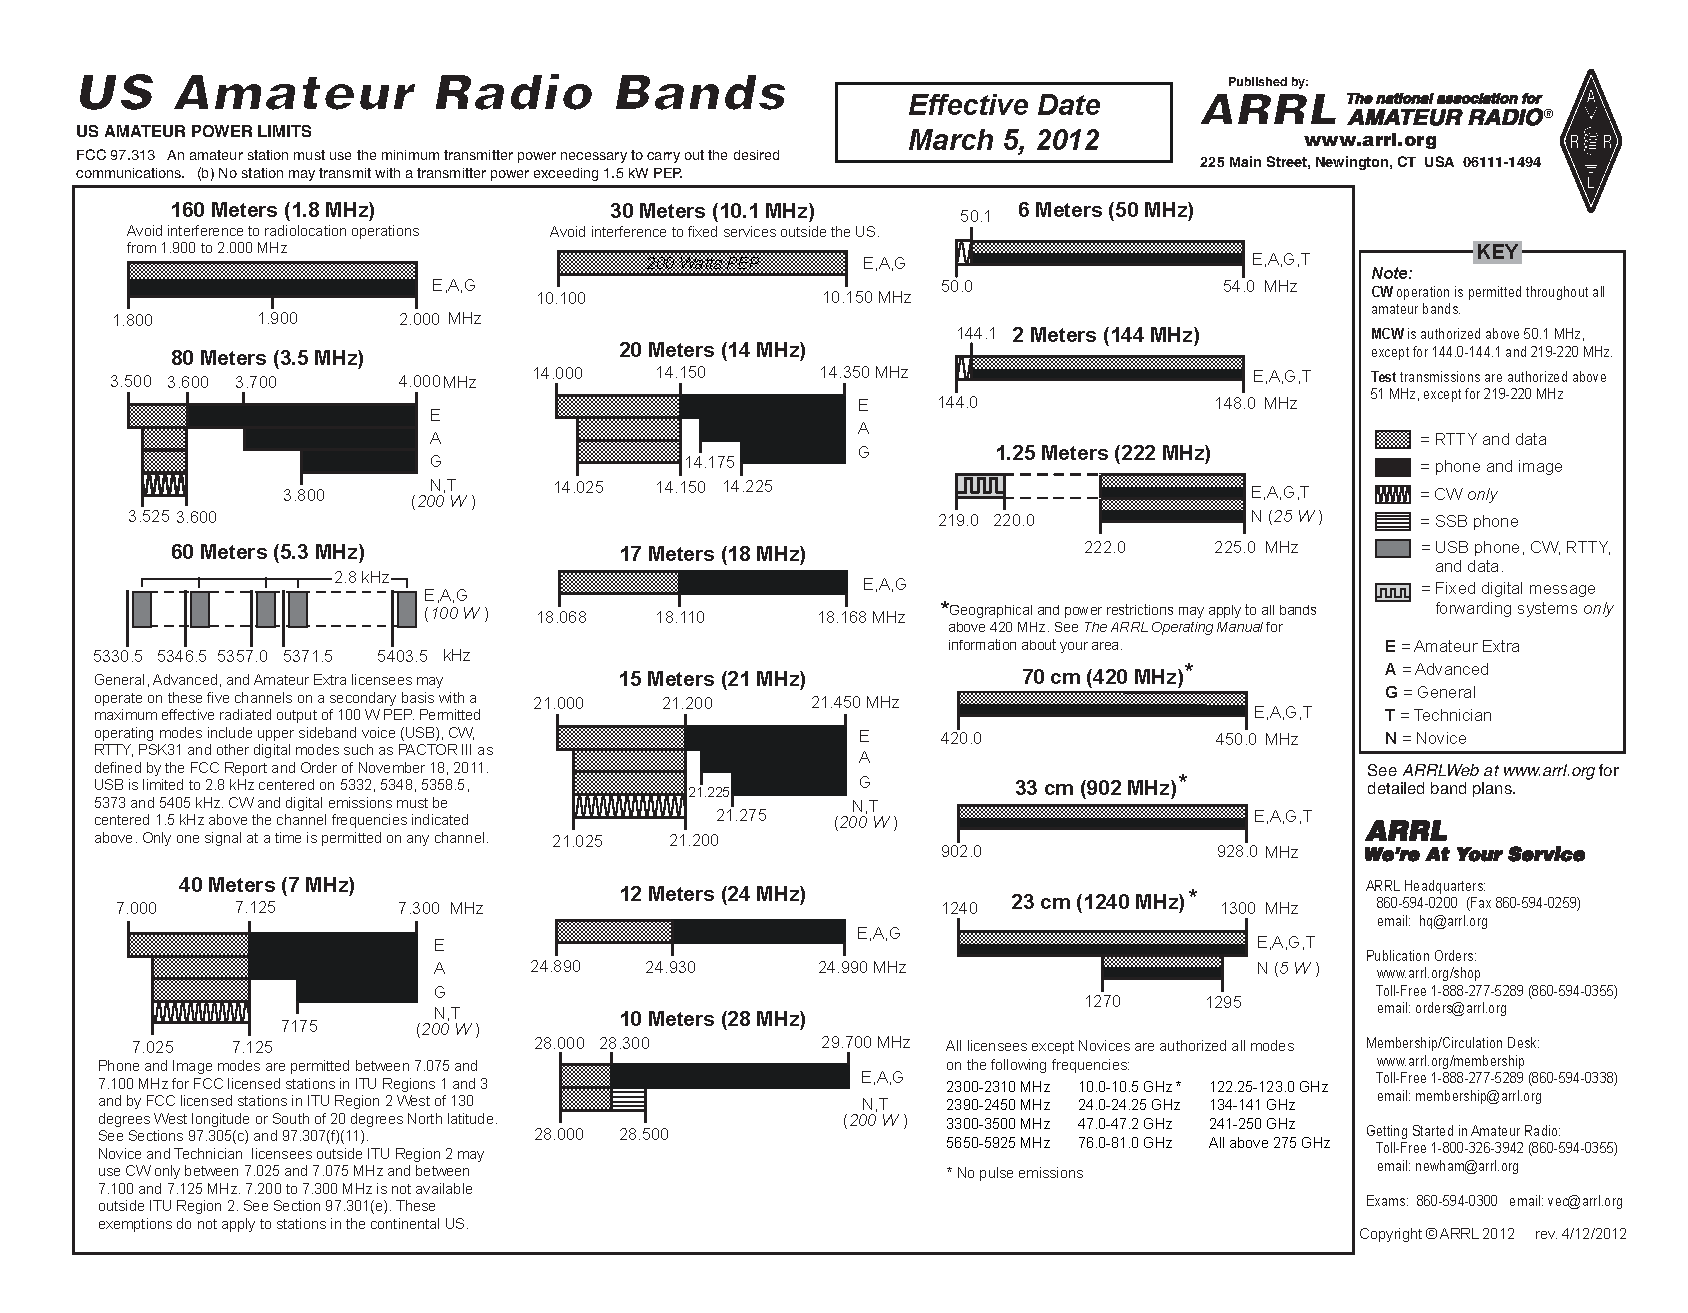
\includepdf[landscape=true]{hambands_bw.pdf} % http://www.arrl.org/files/file/Regulatory/Band%20Chart/Hambands_bw.pdf
\clearpage


\section{Useful Stations}


\subsection{WWV}
WWV is operated by NIST and broadcasts official U.S.\ Government frequency and time signals.

Frequencies: \SIlist{2.5;5.0;10.0;15.0;20.0}{\MHz}


\subsection{W1AW}
W1AW is operated by the ARRL, and routinely transmits practice sessions and bulletins.

Code Frequencies: \SIlist{1.8025;3.5815;7.0475;14.0475;18.0975;21.0675;28.0675;147.555}{\MHz}

Digital Frequencies: \SIlist{3.5975;7.095;14.095;18.1025;21.095;28.095;147.555}{\MHz}

Voice Frequencies: \SIlist{1.855;3.99;7.29;14.29;18.16;21.39;28.59;147.555}{\MHz}

\begin{table}[tbh]
  \begin{tabular}{l l c c c c c}
    \multicolumn{2}{c}{Local Time}	&			&			&			&			&			\\
    Pacific	&	East				& M			& Tu		& W			& Th		& F			\\
    \midrule
    0600	&	0900				&			& Fast Code	& Slow Code	& Fast Code	& Slow Code	\\
    1300	&	1600				& Fast Code	& Slow Code	& Fast Code	& Slow Code	& Fast Code	\\
    1400	&	1700				& \multicolumn{5}{c}{\cellcolor{gray!10}Code Bulletin}		\\
    1500	&	1800				& \multicolumn{5}{c}{\cellcolor{gray!10}Digital Bulletin}	\\
    1600	&	1900				& Slow Code	& Fast Code	& Slow Code	& Fast Code	& Slow Code	\\
    1700	&	2000				& \multicolumn{5}{c}{\cellcolor{gray!10}Code Bulletin}		\\
    1800	&	2100				& \multicolumn{5}{c}{\cellcolor{gray!10}Digital Bulletin}	\\
    1845	&	2145				& \multicolumn{5}{c}{\cellcolor{gray!10}Voice Bulletin}		\\
    1900	&	2200				& Fast Code	& Slow Code	& Fast Code	& Slow Code	& Fast Code	\\
    2000	&	2300				& \multicolumn{5}{c}{\cellcolor{gray!10}Code Bulletin}		\\
  \end{tabular}
\end{table}



\section{Morse Code}
\begin{center}
  \begin{tabular}{c l r l}
    A	&	\dit\dah			& 0	&	\dah\dah\dah\dah\dah	\\
    B	&	\dah\dit\dit\dit	& 1	&	\dit\dah\dah\dah\dah	\\
    C	&	\dah\dit\dah\dit	& 2	&	\dit\dit\dah\dah\dah	\\
    D	&	\dah\dit\dit		& 3	&	\dit\dit\dit\dah\dah	\\
    E	&	\dit				& 4	&	\dit\dit\dit\dit\dah	\\
    F	&	\dit\dit\dah\dit	& 5	&	\dit\dit\dit\dit\dit	\\
    G	&	\dah\dah\dit		& 6	&	\dah\dit\dit\dit\dit	\\
    H	&	\dit\dit\dit\dit	& 7	&	\dah\dah\dit\dit\dit	\\
    I	&	\dit\dit			& 8	&	\dah\dah\dah\dit\dit	\\
    J	&	\dit\dah\dah\dah	& 9	&	\dah\dah\dah\dah\dit	\\
    K	&	\dah\dit\dah		\\
    L	&	\dit\dah\dit\dit	& . &	\dit\dah\dit\dah\dit\dah	\\
    M	&	\dah\dah			& ,	&	\dah\dah\dit\dit\dah\dah	\\
    N	&	\dah\dit			& !	&	\dah\dit\dah\dit\dah\dah	\\
    O	&	\dah\dah\dah		& ? &	\dit\dit\dah\dah\dit\dit	\\
    P	&	\dit\dah\dah\dit	& /	&	\dah\dit\dit\dah\dit		\\
    Q	&	\dah\dah\dit\dah	& ( &	\dah\dit\dah\dah\dit		\\
    R	&	\dit\dah\dit		& ) &	\dah\dit\dah\dah\dit\dah	\\
    S	&	\dit\dit\dit		& '	&	\dit\dah\dah\dah\dah\dit	\\
    T	&	\dah				& " &	\dit\dah\dit\dit\dah\dit	\\
    U	&	\dit\dit\dah		& + &	\dit\dah\dit\dah\dit		\\
    V	&	\dit\dit\dit\dah	& - &	\dah\dit\dit\dit\dit\dah	\\
    W	&	\dit\dah\dah		& = &	\dah\dit\dit\dit\dah		\\
    X	&	\dah\dit\dit\dah	& : &	\dah\dah\dah\dit\dit\dit	\\
    Y	&	\dah\dit\dah\dah	& ; &	\dah\dit\dah\dit\dah\dit	\\
    Z	&	\dah\dah\dit\dit	& @ &	\dit\dah\dah\dit\dah\dit	\\
  \end{tabular}
\end{center}

\begin{center}
  \begin{tabular}{l c l}
    pause					&	\prosign{BT}	&	\dah\dit\dit\dit\dah					\\
    back to other station	&	\prosign{AR}	&	\dit\dah\dit\dah\dit					\\
    end transmission		&	\prosign{SK}	&	\dit\dit\dit\dit\dah\dit				\\
    break					&	BK				&	\dah\dit\dit\dit \quad \dah\dit\dah		\\
    go ahead / over			&	K				&	\dah\dit\dah							\\
    over (specific station)	&	KN				&	\dah\dit\dah \quad \dah\dit				\\
    shutting down			&	CL				&	\dah\dit\dah\dit \quad \dit\dah\dit\dit	\\
  \end{tabular}
\end{center}



\section{Common Q Codes}
\begin{center}
  \begin{tabular}{c l l}
    Code	& Question								& Answer / Advice / Order				\\
    QRL		& Are you busy?							& I am busy. Don't interfere.			\\
    QRM		& Are you being interfered with?		& I am being interfered with.			\\
    QRN		& Are you troubled by static noise?		& I am troubled by static.				\\
    QRO		& Should I increase power?				& Increase power.						\\
    QRP		& May I decrease power?					& Decrease power.						\\
    QRQ		& May I send faster?					& Send faster.							\\
    QRS		& Should I send more slowly?			& Send more slowly.						\\
    QRT		& Should I stop transmission?			& Stop transmission						\\
    QRU		& Do you have anything for me?			& I have nothing for you.				\\
    QRV		& Are you ready?						& I am ready.							\\
    QRX		& When will you call again?				& I will call you again. (time, freq)	\\
    QRZ		& Who (else) is calling?				& You are being called by \ldots		\\
    QSB		& Is my signal strength varying?		& Your signal strength is varying.		\\
    QSK		& Shall I continue transmitting?		& Continue. I will interrupt if needed.	\\
    QSL		& Can you acknowledge receipt?			& I acknowledge receipt.				\\
    QSO		& Can you communicate with \ldots?		& I can communicate with \ldots.		\\
    QSY		& Shall I change frequency to \ldots?	& Change frequency to \ldots.			\\
    QTH		& What is your location?				& My location is \ldots.				\\
    QST		&										& Essentially ``CQ ARRL''				\\
  \end{tabular}
\end{center}
  

\end{document}
